\section{The archive} 

At the time of writing, the full ULTRACAM archive is still undergoing analysis by the automated pipeline. At present \emph{347} nights, out of a total of \emph{406}, have been processed and are available for viewing on a web server hosted at the University of Warwick. Of these processed nights, approximately \emph{xx} have been investigated for variability. At the moment, the investigation is performed by a visual check on the light-curve. The web interface is designed so that it is easy for the viewer to examine the light-curves of all of the objects systematically. The user-interface allows the users to see each light curve in turn by pressing the 'right' and 'left'  arrow keys on the keyboard. More information on how to use this interface can be found in the User Manual at appendix ~\ref{chap:usermanual}. 

\section{Data quality}

\subsection{Photometric calibration}
The main purpose of this MSc project was to establish a process for automatically reducing the light-curves for all objects in the data archive rather than to focus on accurate and well-calibrated measurements. The diverse nature of the dataset means that it is not trivial to write a purely automated algorithm that can perform fully calibrated measurements. 

Correct calibration of the photometry for ULTRACAM requires to the following steps:
\begin{itemize}
  \item Using \emph{flat fields} to take into account the varying sensitivity of the individual pixels of the CCD detector. 
  \item Subtracting \emph{bias} frames from each image to remove the additional counts caused by having a non-zero bias on the CCD. 
  \item Using a \emph{standard star} to calculate the offset magnitude required to calibrate to the standard magnitude system. For ULTRACAM these are usually Sloan u, g, r, i magnitudes.
  \item Computing the \emph{atmospheric extinction} for the night by fitting extinction curves for a number of bright objects that have been measured over a range of airmass. 
\end{itemize}
During a typical night at the telescope, the observers will take steps to ensure that there are sufficient data to perform this calibration. They will take several bias frames, flat-fields and will observe standard stars. When the reduction is performed later, these various datasets will be combined to calibrate the photometry of the target objects. 

The automated pipeline built for this project lacks the ability to correctly identify the appropriate bias readings, flat-fields and standard stars that should be used for photometric calibration. This requires human intervention. Therefore, this step is skipped altogether. The magnitudes and flux counts produced by the automated pipeline are \emph{not} calibrated and will differ from their true values by a certain offset.

It is possible to take the output of the automated pipeline and calibrate the photometry, but, at the moment, this is a manual process. 

\subsection{Comparison of the 2 pipelines}
Since the ULTRACAM already has a well-established data reduction pipeline, it is useful to compare the results of this pipeline with the new, automated one built in this project. As mentioned above, the automated pipeline does not perform calibrated photometry, but we can still compare the non-calibrated photometry to get an estimate of how well our new pipeline performs.

In order to do this, we chose a run of a target object that has often been observed with the ULTRACAM. The object is \emph{NN Ser}, a white-dwarf, M-dwarf eclipsing binary. The specific run in question is \emph{2013-07-13/run111}.

Running the automated pipeline on this run is achieved by simply typing: \texttt{runbuilder.py 2013-07-13/run111} on the command line. Please refer to the user manual in appendix \ref{chap:usermanual} for instructions on how to install and run the pipeline.  The reduction takes about 5 minutes of processing time running on a standard desktop machine in the University of Warwick Astronomy department. The output of this reduction can be seen at \url{http://deneb.astro.warwick.ac.uk/phrnaw/sitedev/2013-07-13/run111.html}.

\begin{figure}
\centering
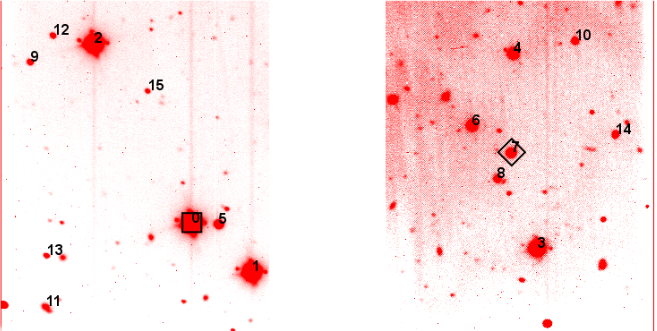
\includegraphics[width=120mm]{images/2013-07-13-run111-r-withlabels.png}
\caption{Snapshot taken from the automated pipeline browser for 2013-07-13/run111. The target, {NN Ser} is labeled object `7' in the image. This is a stacked image from the 'red' CCD with the Sloan 'i' filter. }
\label{fig:nnserfield}
\end{figure}

\begin{figure}
\centering
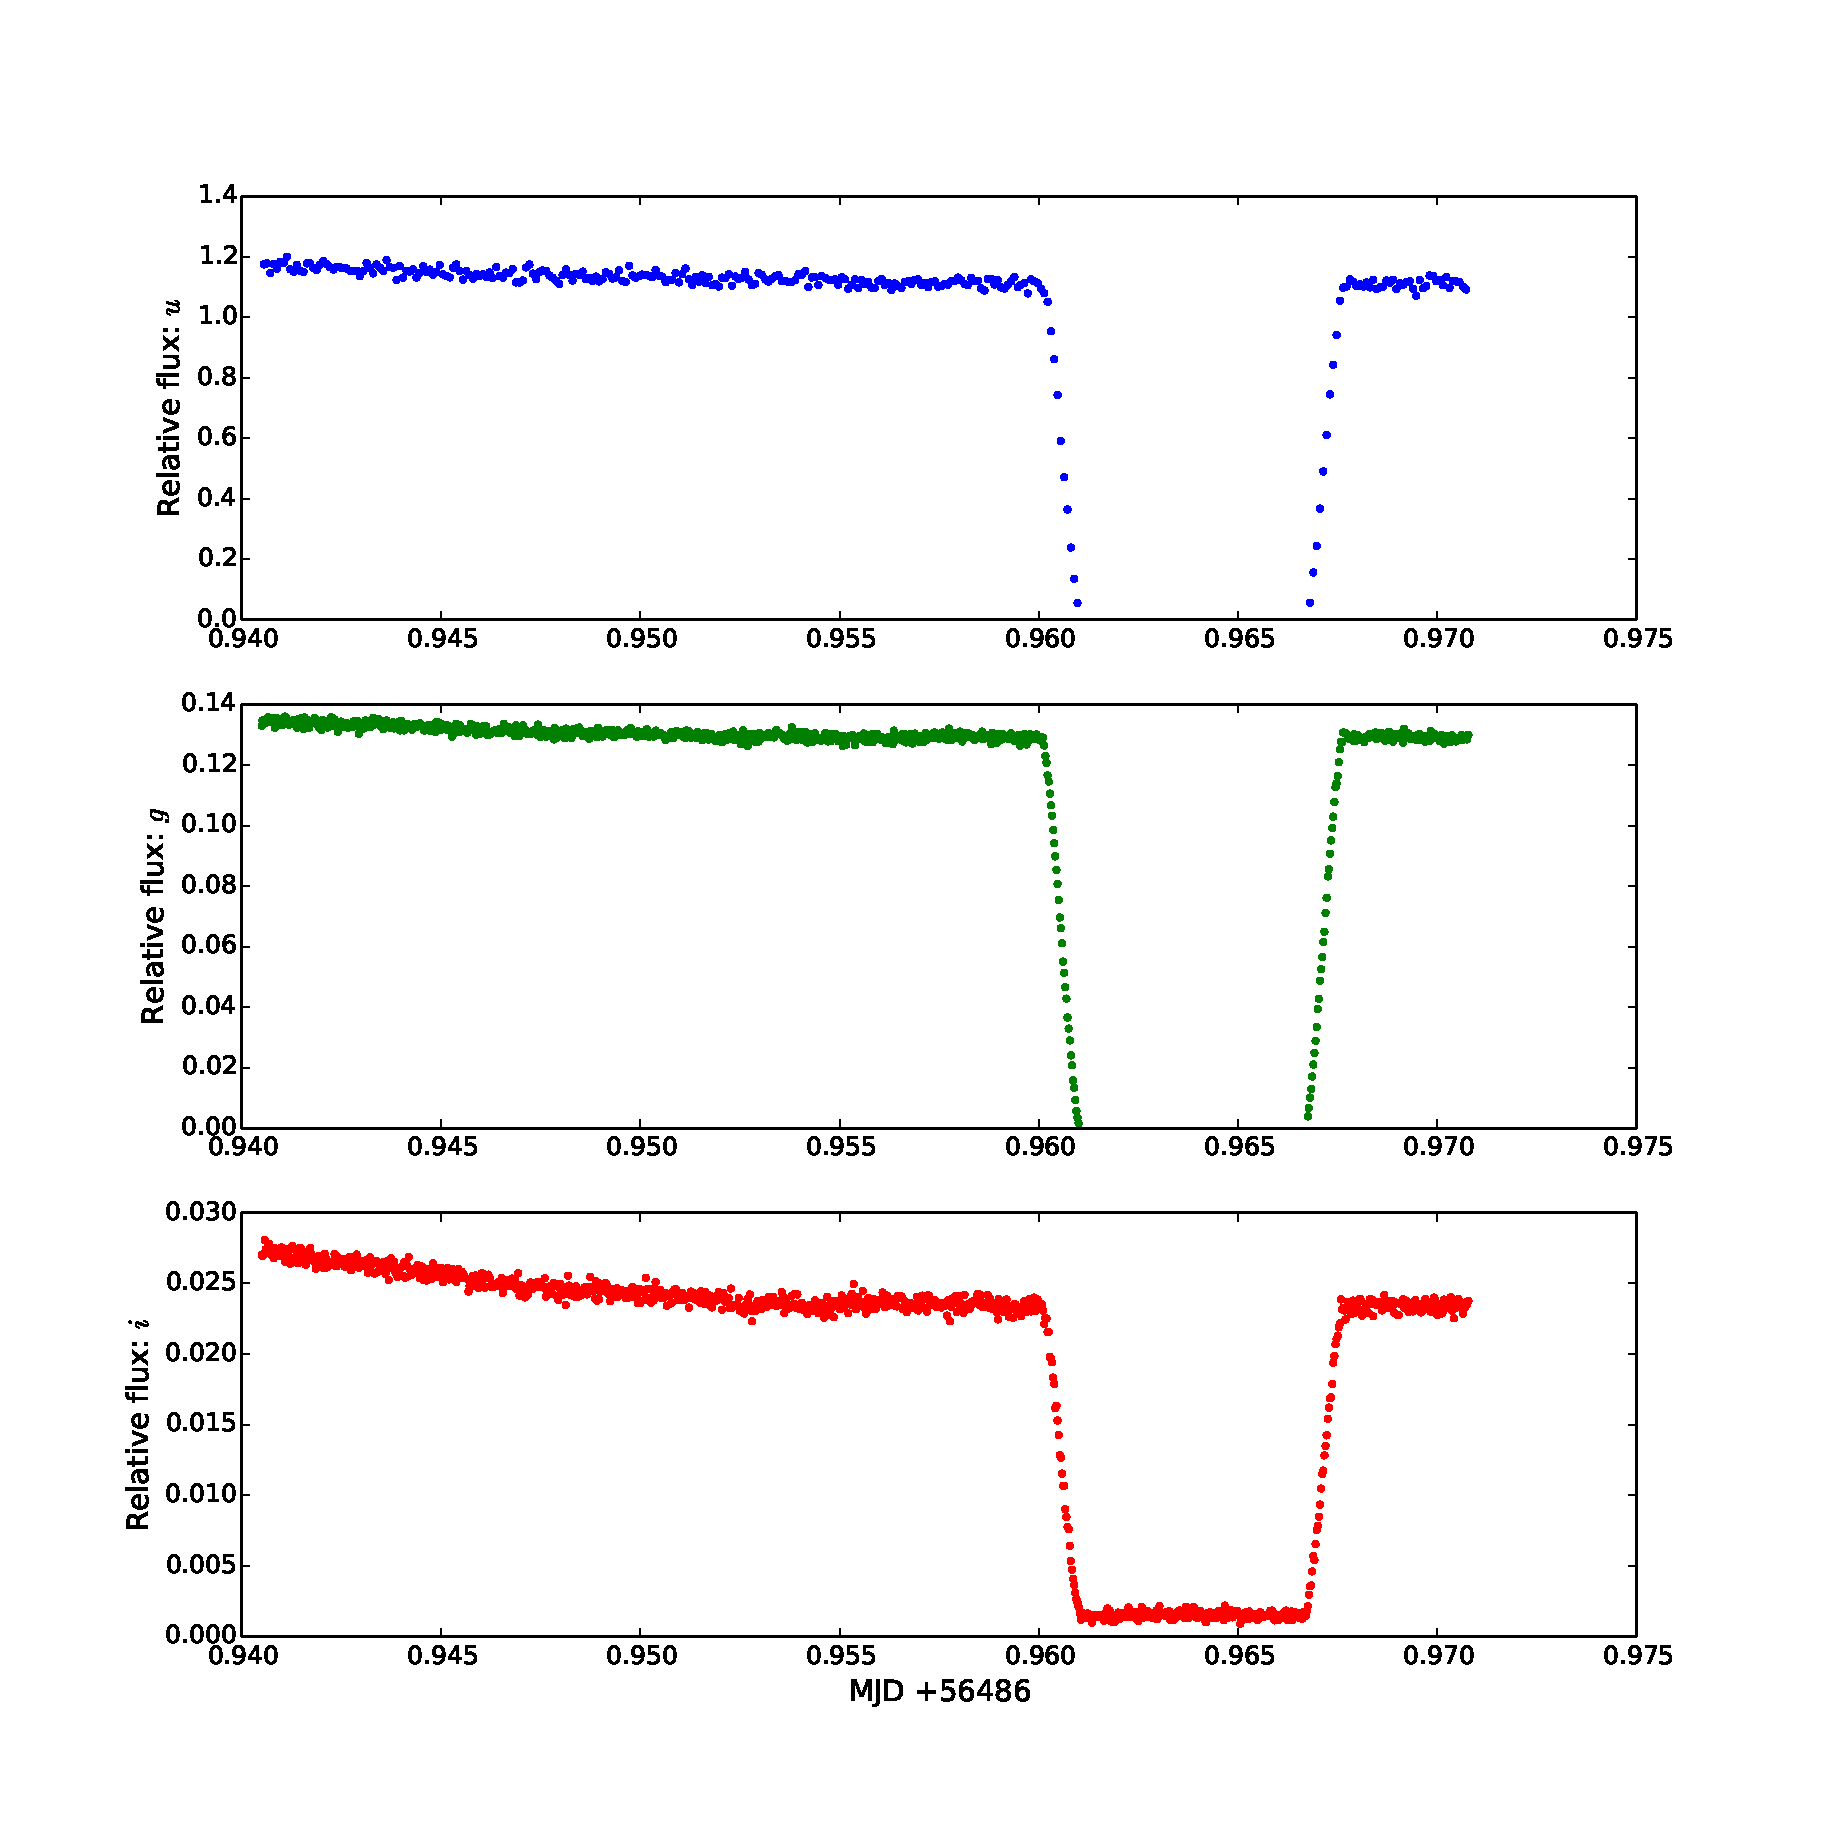
\includegraphics[width=140mm]{images/nnser_lightcurve_automated.eps}
\caption{Light curve of the target object, NN Ser produced using the \emph{automated pipeline}. The vertical axis is the raw flux measurements calculated by SExtractor.}
\label{fig:nnserlightcurveautomated}
\end{figure}

\begin{figure}
\centering
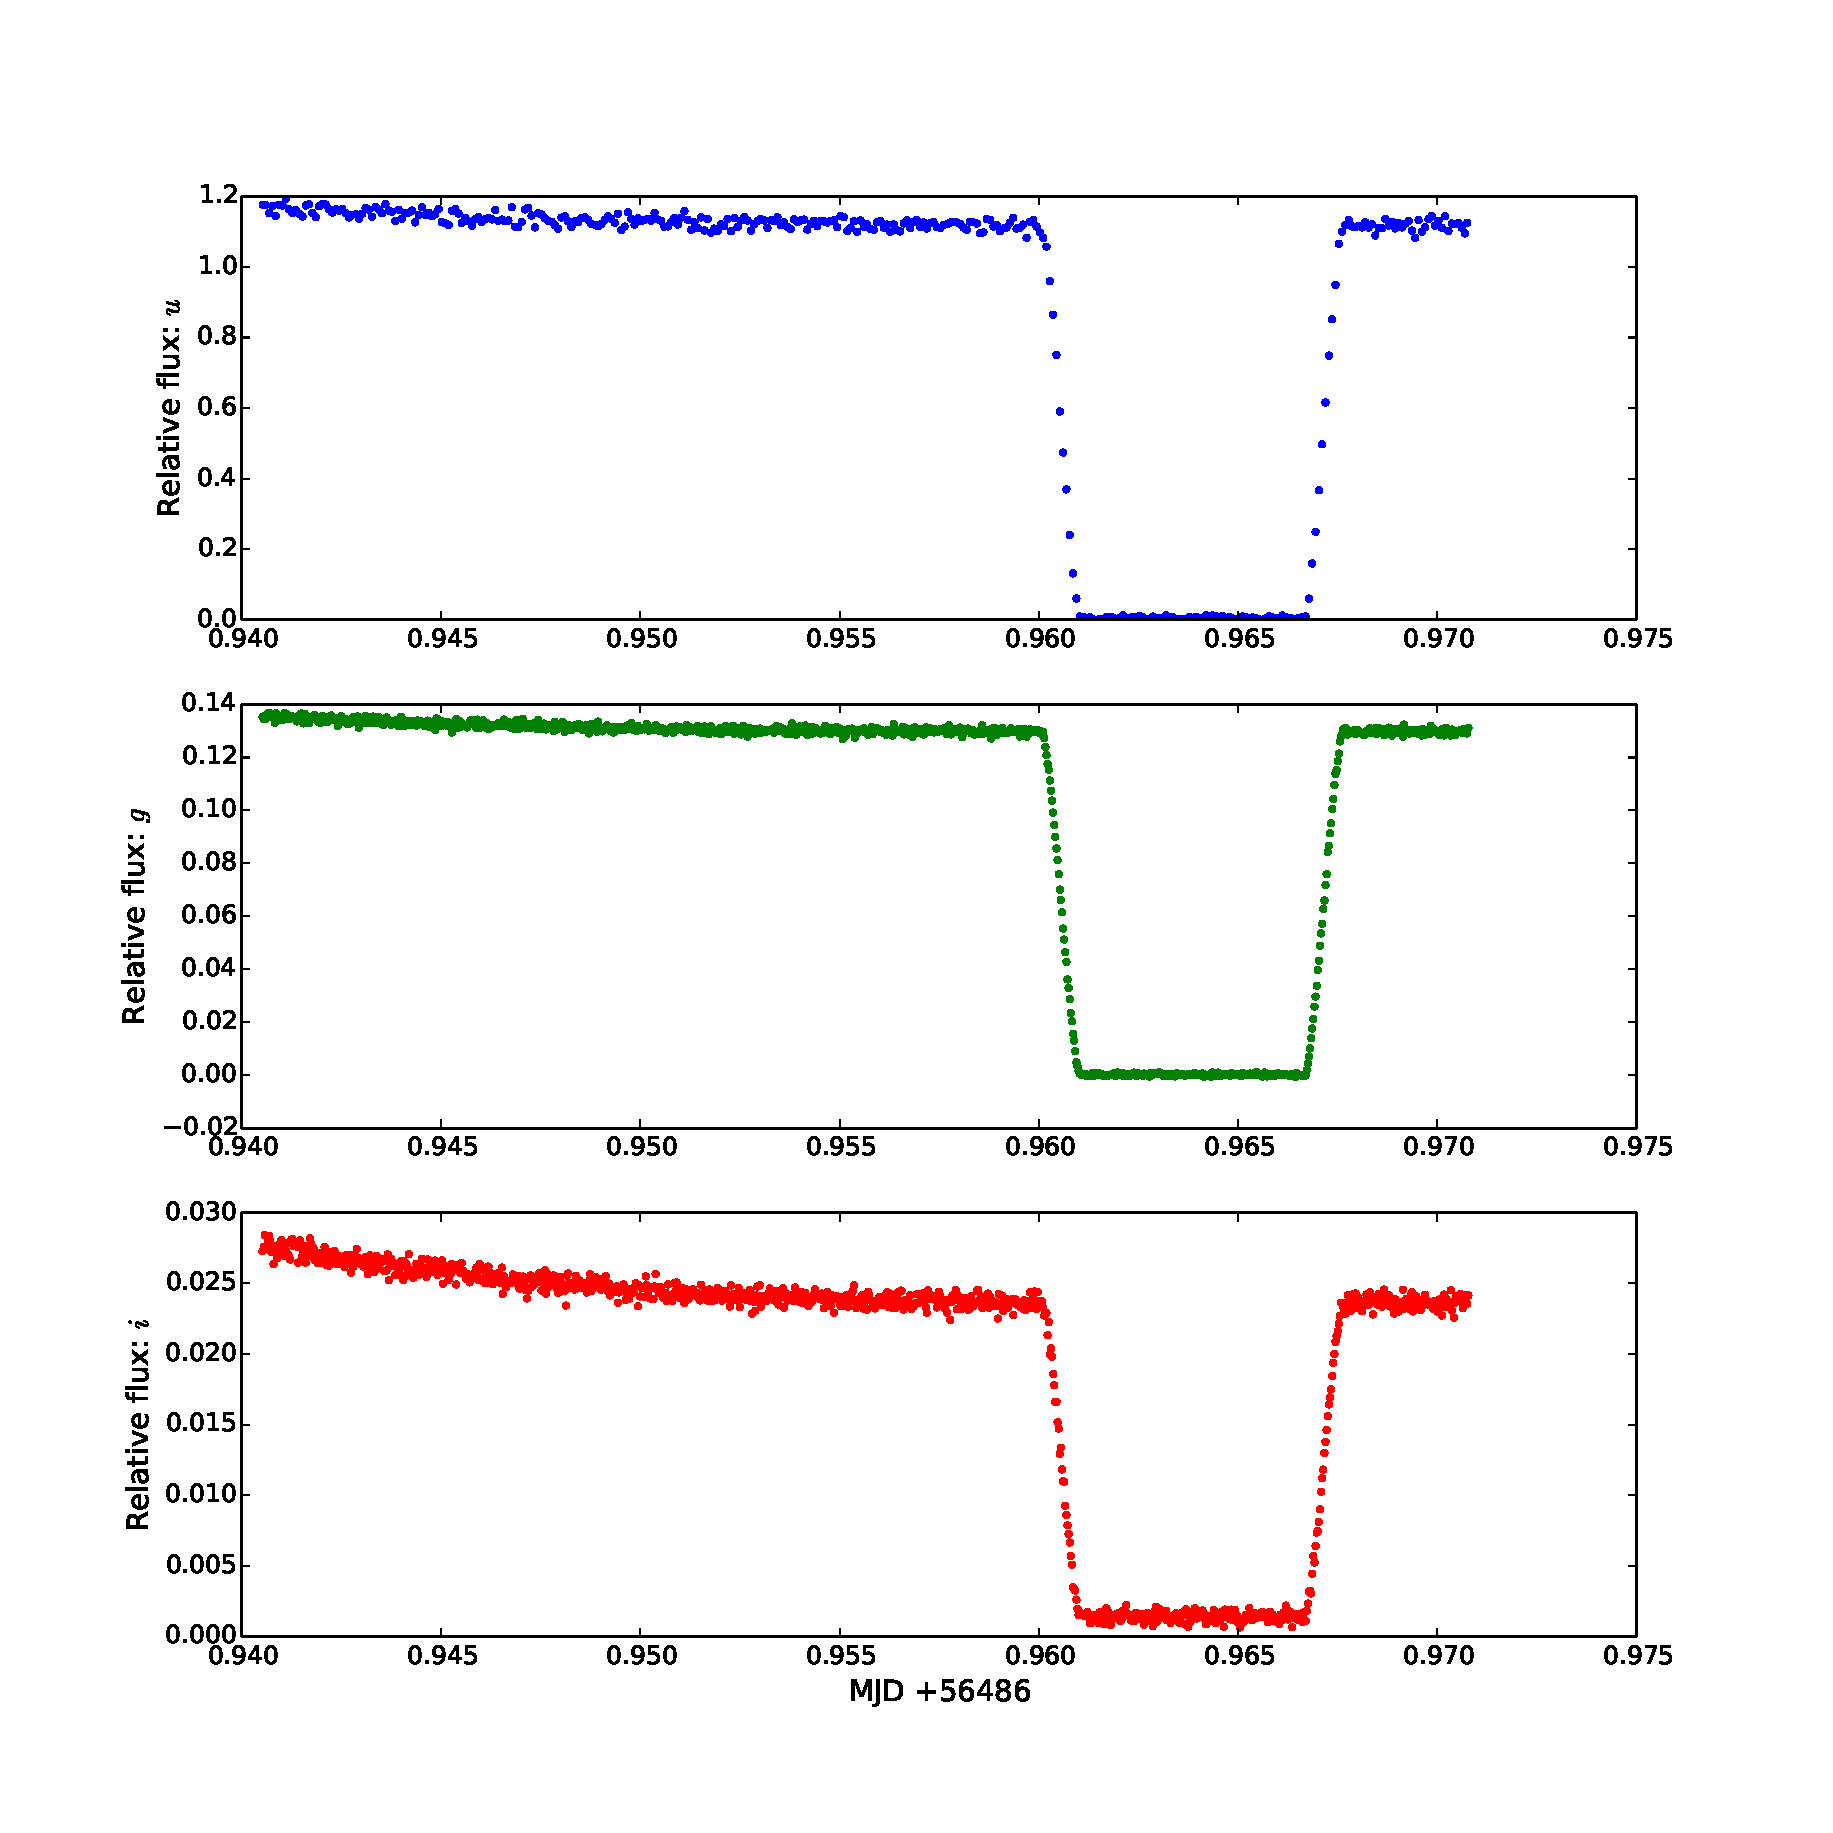
\includegraphics[width=140mm]{images/nnser_lightcurve_tom.eps}
\caption{Light curve of the target object, NN Ser, produced using the \emph{standard pipeline}. }
\label{fig:nnserlightcurvetom}
\end{figure}

The light-curves in figures \ref{fig:nnserlightcurveautomated} and \ref{fig:nnserlightcurvetom} are a good demonstration of the reduction of an interesting eclipse, but, in order to perform a comparison of the two pipelines, it makes more sense to choose two objects in this run that we can assume are \emph{constant} objects. The two objects we have chosen are the two brightest objects in the field and are labeled '0' and '1' in figure \ref{fig:nnserfield}. We are making the assumption that these two objects are of constant brightness. Since we will be comparing the \emph{differential} photometry of these two objects, in other words, the ratio $Counts_{0}/Counts_{1}$, any variations due to the systematic effects of the observation itself, such as atmospheric transmission, etc will be equivalent for both objects. Figures \ref{fig:differentialauto} and \ref{fig:differentialtrad} show the differential photometry for the two pipelines. Both of the pipelines have consistent values and agree with each to well within 1 standard deviation.

\begin{table}[ht]
  \label{tab:differential}
  \caption{Table showing the statistics of the differential photometry produced by dividing the flux counts for object '0' by the flux counts for object '1'.}
  \centering
  \begin{tabular}{|l|r|r|}
    \hline
    Filter & Traditional pipeline & Automated pipeline  \\
           &  $mean[std. dev]$    & $mean[std. dev]$ \\
    \hline
    'i'    & 1.2521[0.0036]       & 1.2523[0.0034] \\
    'g'    & 1.2247[0.0045]       & 1.2240[0.0042]\\
    'u'    & 1.264[0.019]         & 1.259[0.017] \\
    \hline
   \end{tabular}
\end{table}

\begin{figure}[!h]
\centering
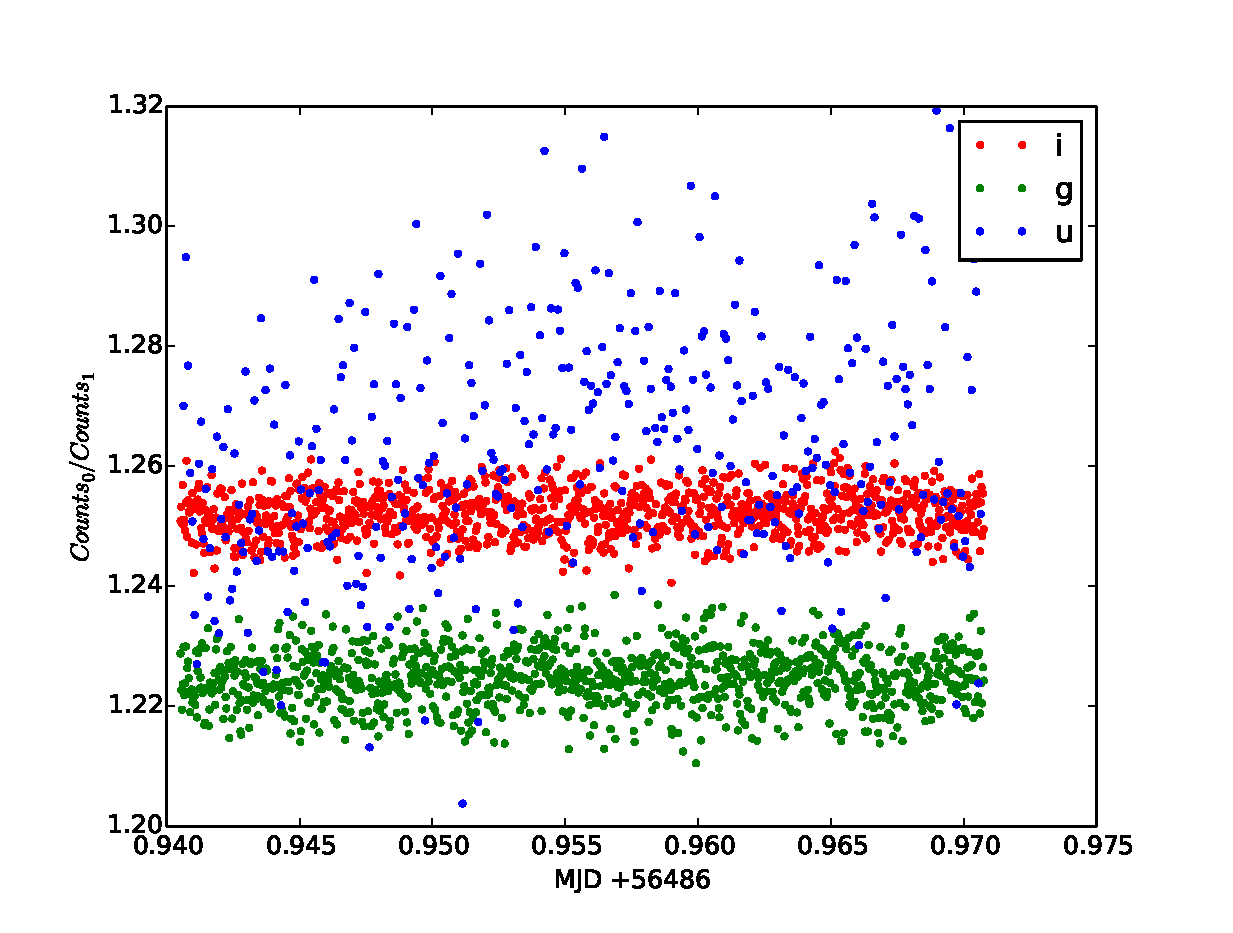
\includegraphics[width=140mm]{images/differential_auto.eps}
\caption{The light-curve of the flux ratio of object '0' and object '1' as labelled in figure \ref{fig:nnserfield} produced by the \emph{automated} pipeline. The vertical axis shows the flux counts for object '0' divided by the flux counts for object '1'. Both of the objects are assumed to be constant sources. }
\label{fig:differentialauto}
\end{figure}

\begin{figure}[!h]
\centering
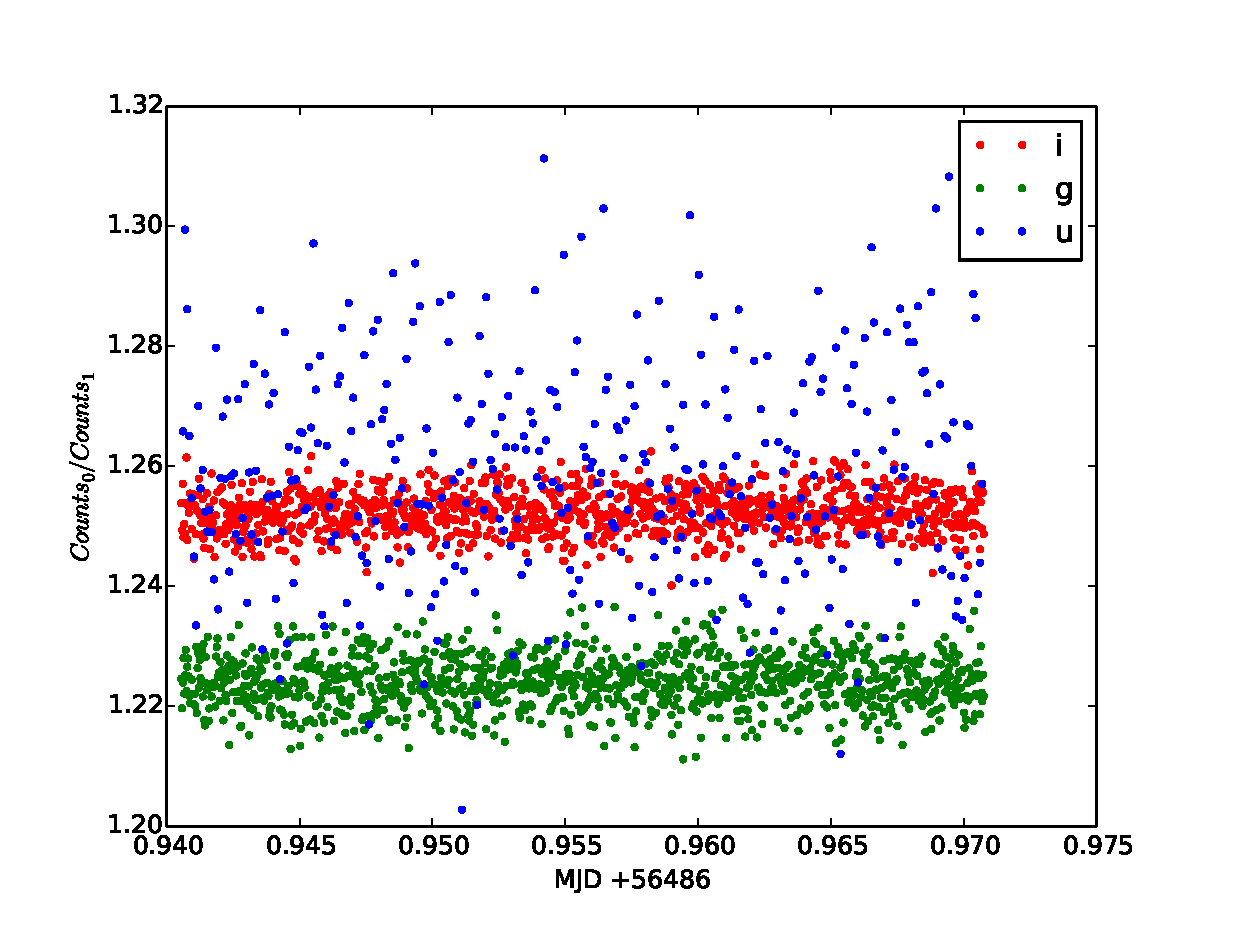
\includegraphics[width=140mm]{images/differential_trad.eps}
\caption{The light-curve of the flux ratio object '0'  object '1' as labelled in figure \ref{fig:nnserfield} produced by the \emph{traditional} pipeline. The vertical axis shows the flux counts for object '0' divided by the flux counts for object '1'. Both of the objects are assumed to be constant sources. }
\label{fig:differentialtrad}
\end{figure}

\subsection{Apertures}
Since the automated pipeline relies on the third party software, SExtractor, to determine the apertures on each frame, objects that do not meet the required signal to noise ratio on any particular frame will not be detected and therefore have no aperture defined for that frame. This means that objects that fade or are generally quite faint, might 'disappear' on some frames and then 're-appear' on subsequent frames. The tracking algorithm allows a 're-appearing' object to be identified with an object that appeared on previous frames provided that the pixel location is roughly similar. An illustration of this can be seen in figures \ref{fig:nnserlightcurveautomated} and \ref{fig:nnserlightcurvetom} where the automated pipeline 'loses' the target object in the 'g' and 'u' bands after the ingress of the primary eclipse, but picks it up again at the start of egress. In contrast, the traditional reduction pipeline can have apertures that are linked to other objects in the field and can therefore continue to calculate flux in the aperture for the target even if the target is barely detectable above the sky background.

\section{Colour-Colour plots}
Although the automated pipeline does not perform a calibration of the magnitudes of the objects, by using standard stars and extinction corrections, it is still possible to create colour-colour diagrams provided that we are not concerned with the correct offsets for our $(u-g)$ and $(g-r)$ axes. For a few selected runs, where we have > 100 objects clearly identified for the run, we can produce non-calibrated colour-colour diagrams. 

\begin{figure}
\centering
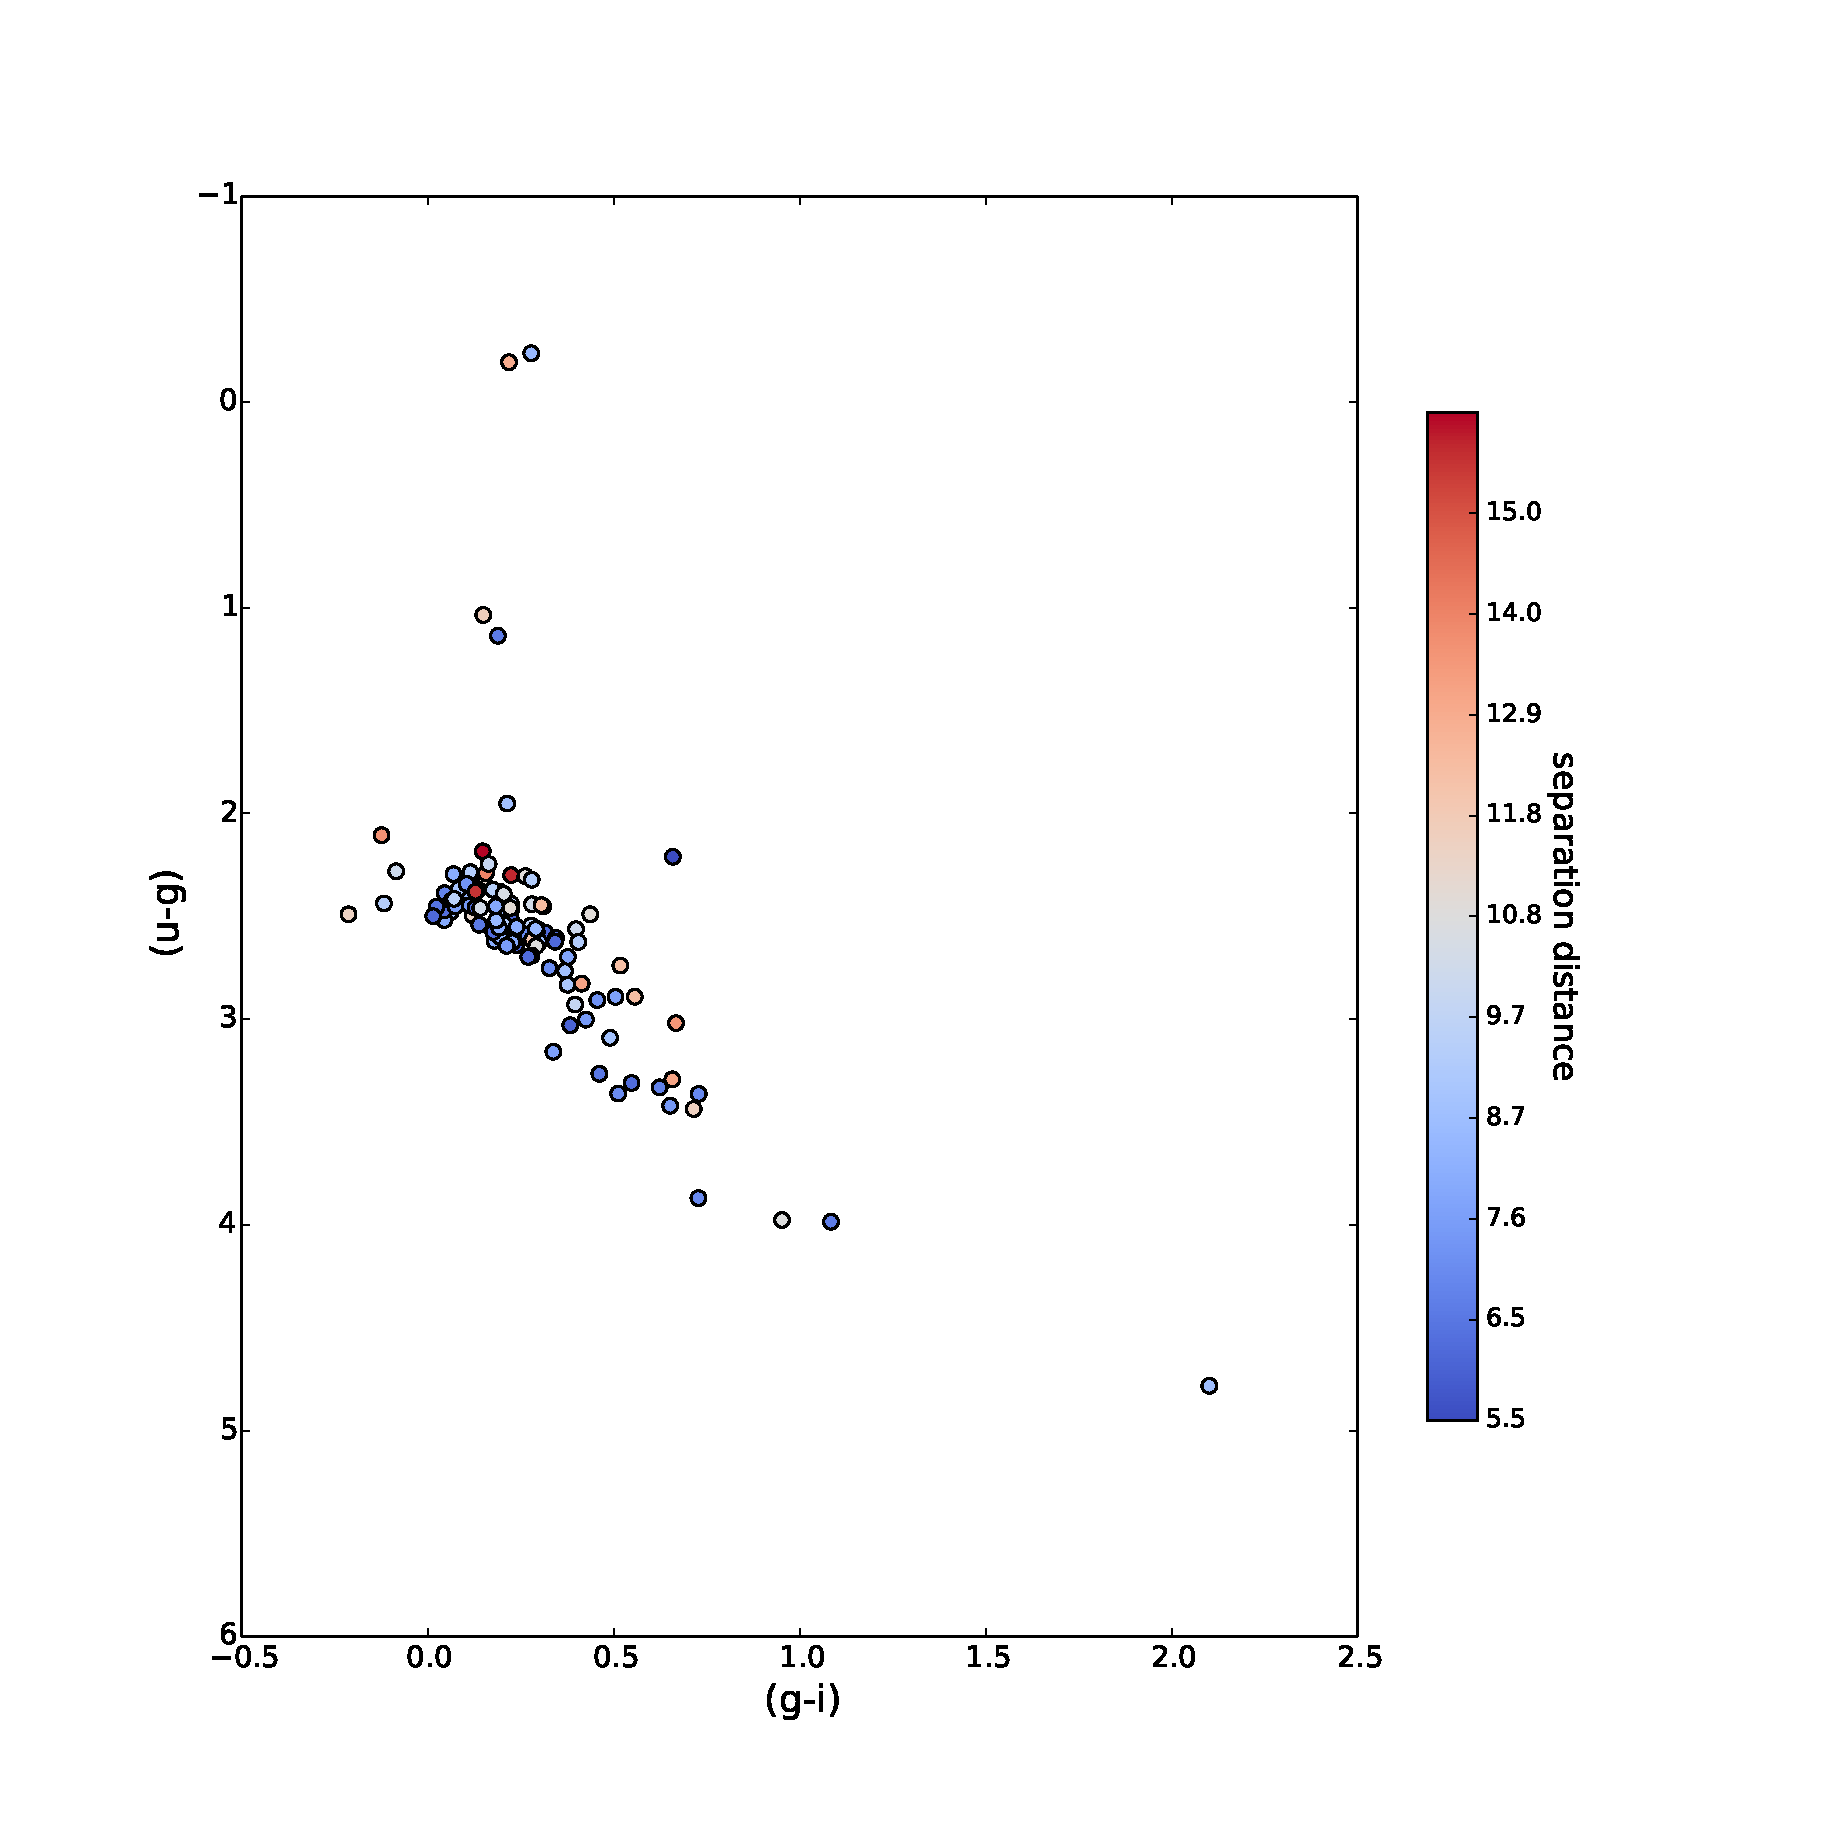
\includegraphics[width=120mm]{images/2013-07-21-run010-2colour.eps}
\caption{The colour-colour plot of run: \emph{2013-07-21/run010}. The plot contains 110 objects located near the Kepler exoplanet host KIC5115978, which is slightly out of the galactic plane. The field contains The offsets on the x and y axes are both arbitrary as the photometry has not been calibrated to photometric standards.}
\label{fig:differentialtrad}
\end{figure}

\begin{figure}
\centering
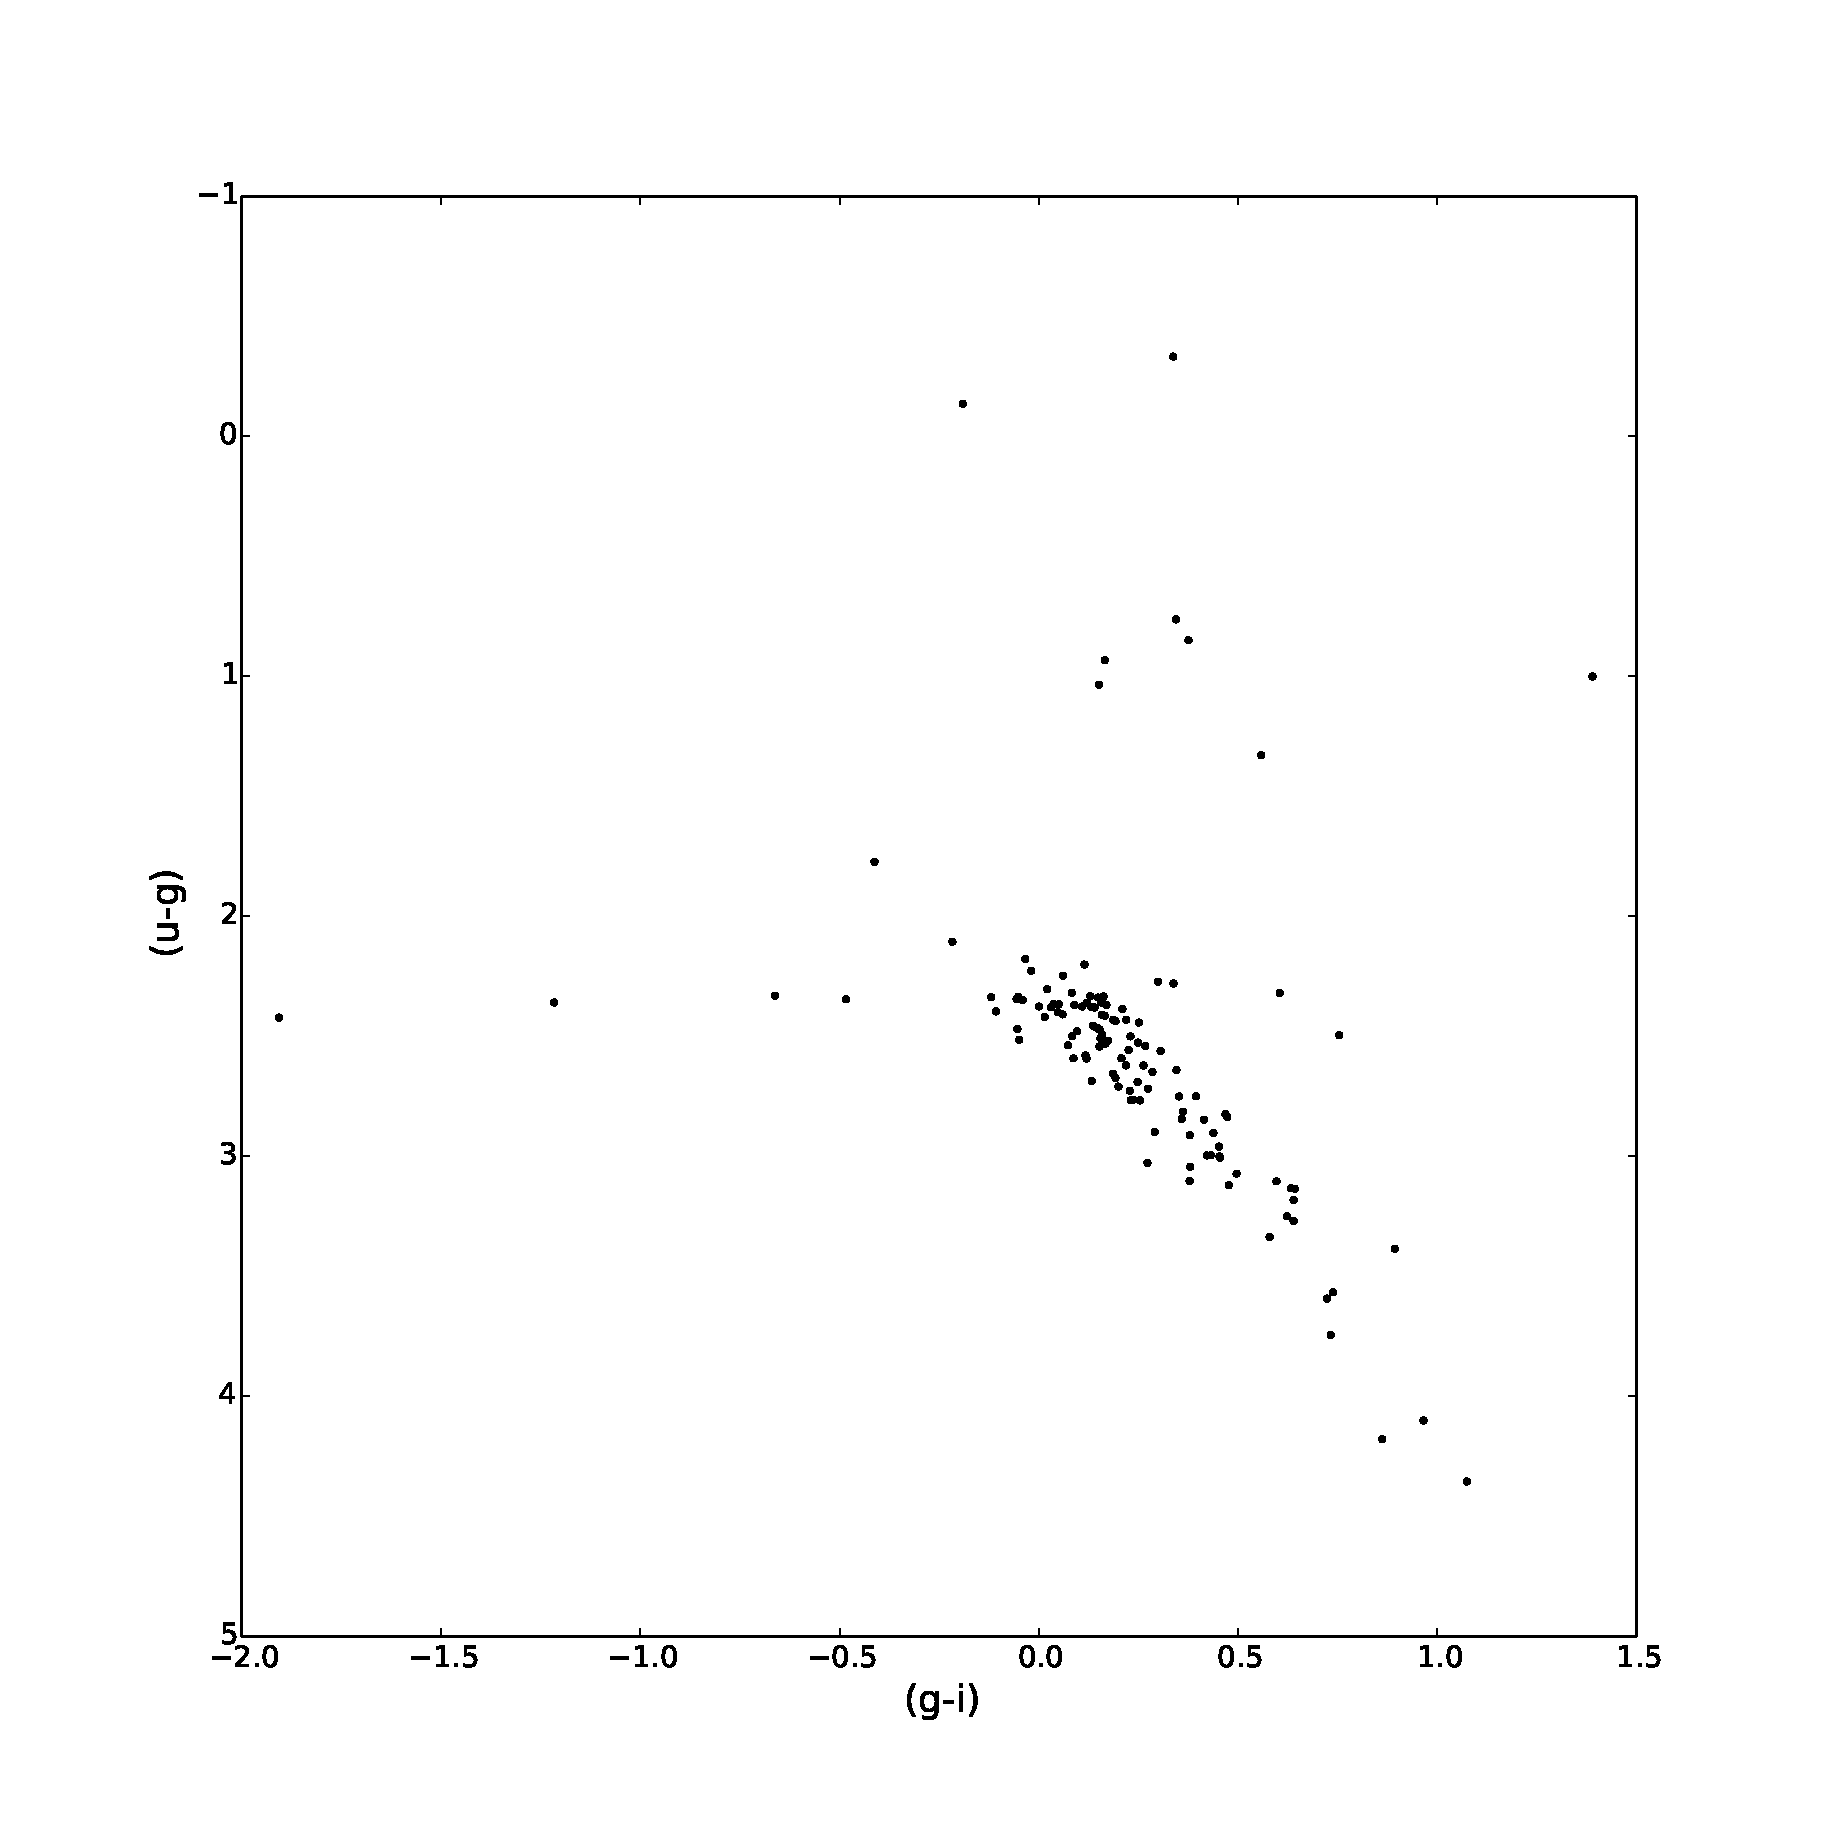
\includegraphics[width=120mm]{images/2013-07-21-run011-2colour.eps}
\caption{The colour-colour plot of run: \emph{2013-07-21/run011}. The offsets on the x and y axes are both arbitrary as the photometry has not been calibrated to photometric standards.}
\label{fig:differentialtrad}
\end{figure}


\begin{figure}
\centering
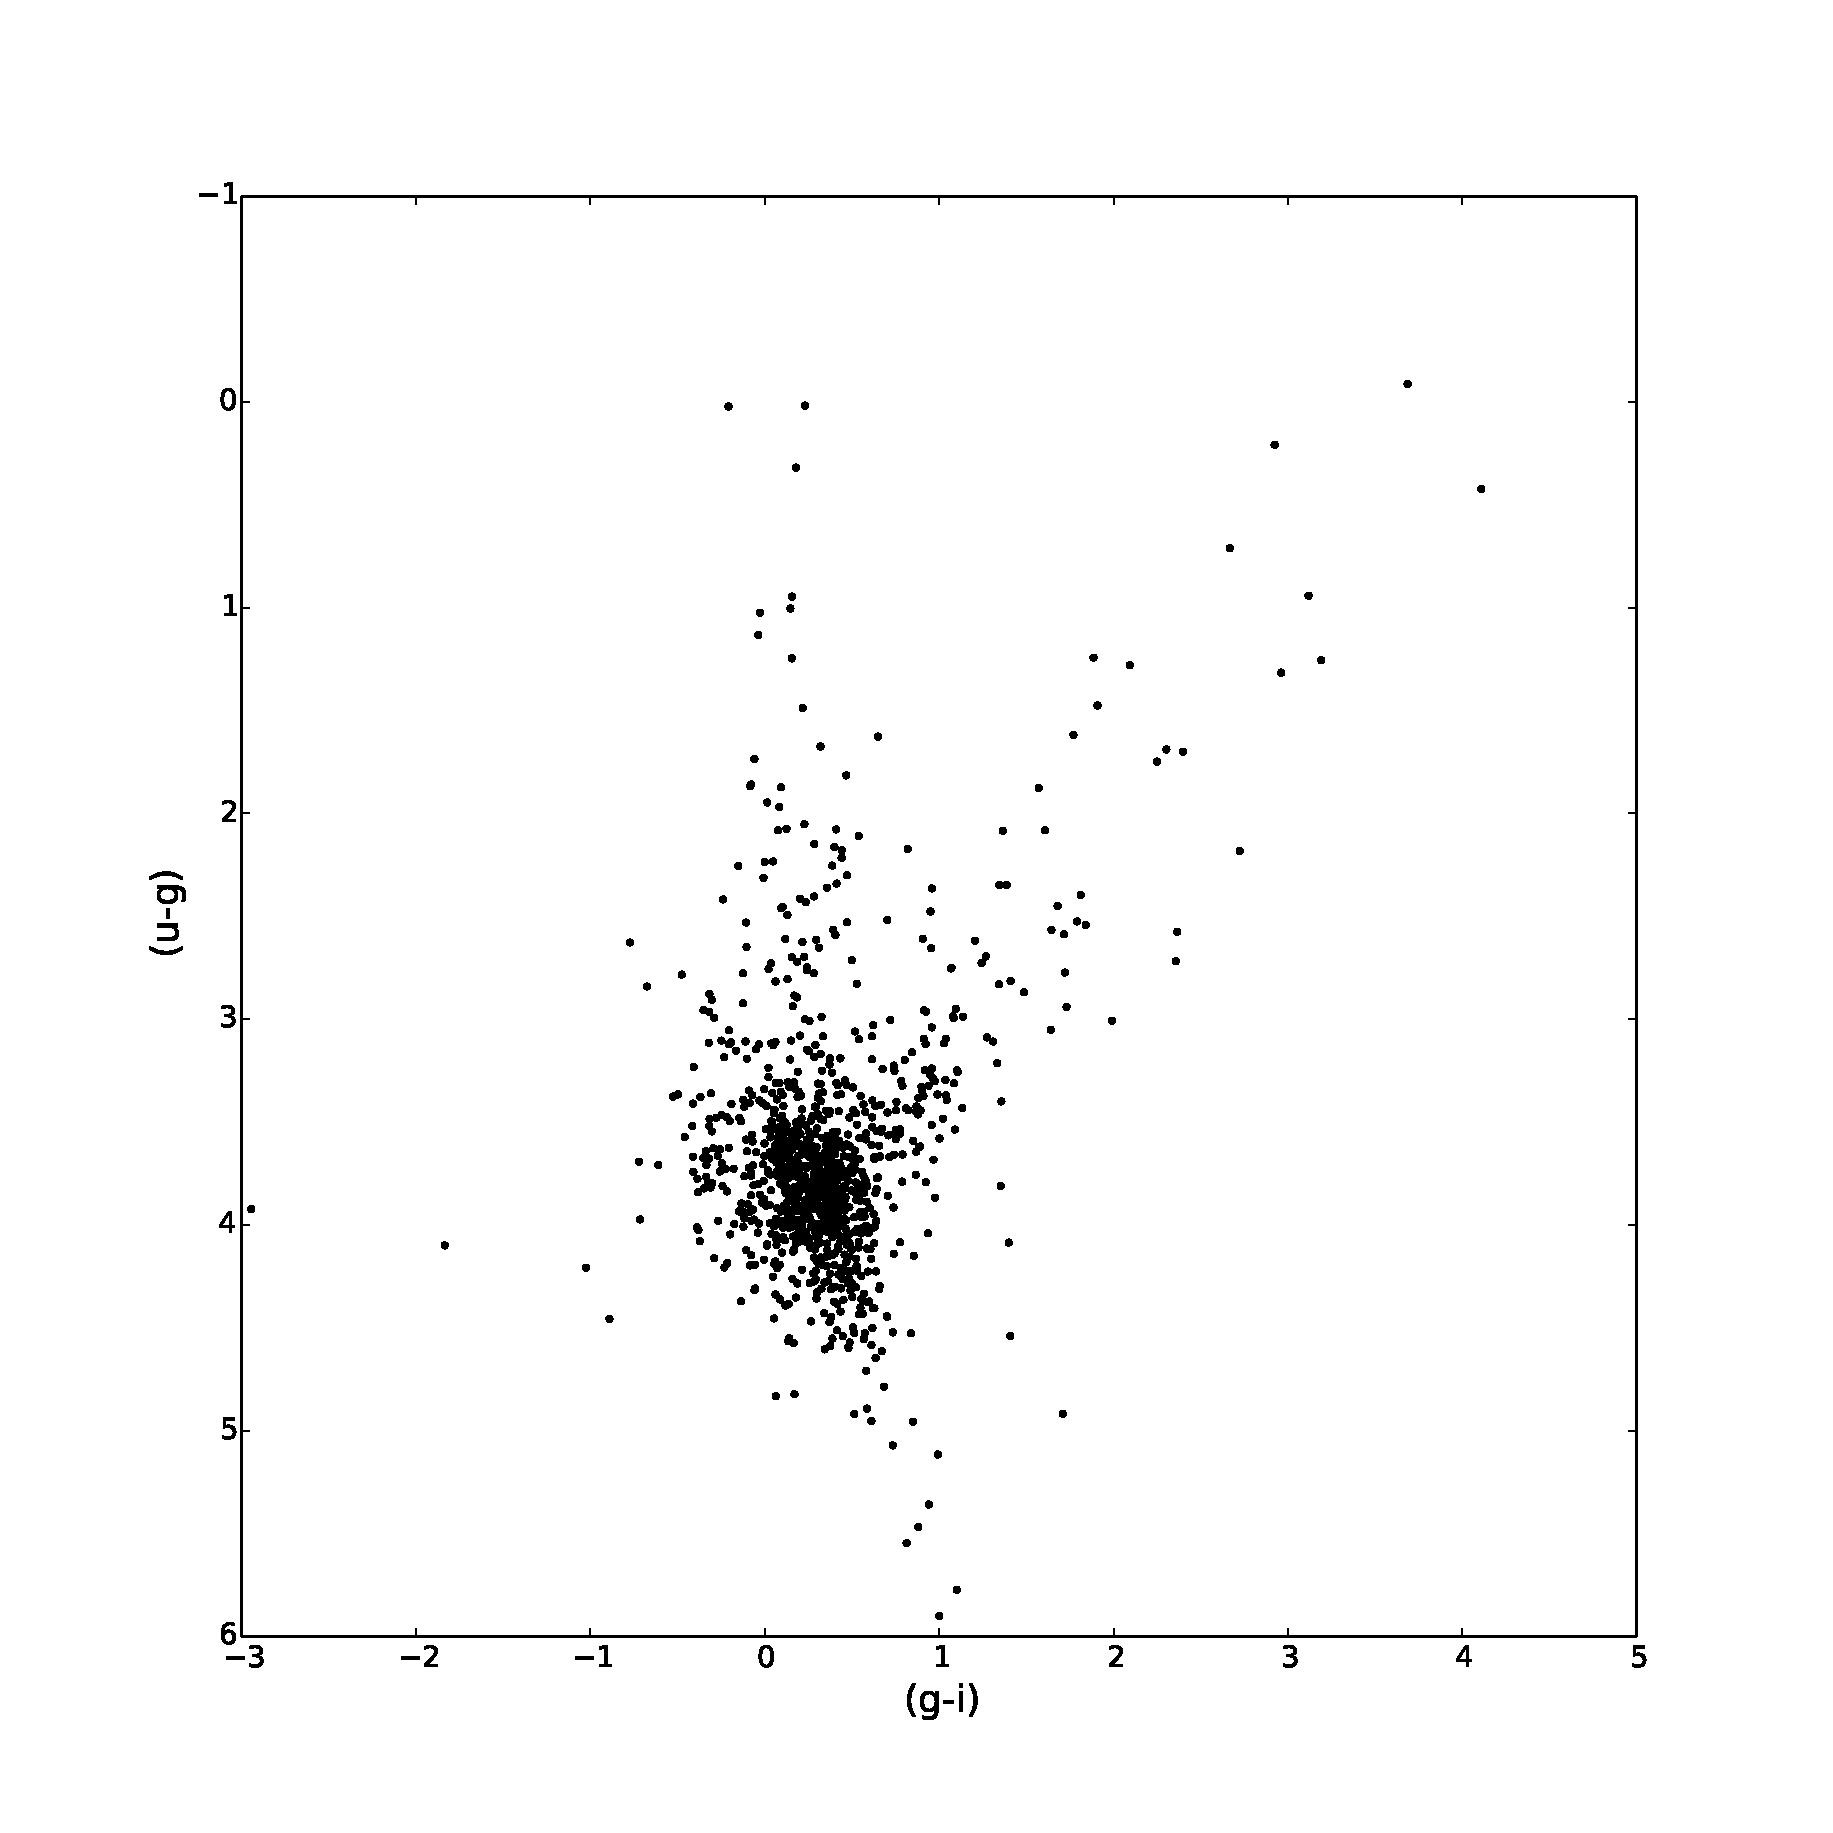
\includegraphics[width=120mm]{images//2011-04-22-run019-omegacen-2colour.eps}
\caption{The colour-colour plot of run: \emph{2011-04-22/run019}. The field contains 1088 objects identified in edge of the globular cluster \emph{Omega Centaurus}. The offsets on the x and y axes are both arbitrary as the photometry has not been calibrated to photometric standards. The extreme blue outliers are errors caused by the pipeline mis-identifying objects across the three channels.}
\label{fig:differentialtrad}
\end{figure}

It should be added that it is possible to produce calibrated colour-colour diagrams from the automated pipeline, if we manually perform the calibration and correct our figures. \emph{Comment: We can include Matthew's colour colour plot here.} 
